\documentclass{article}
\usepackage{tikz}
\usetikzlibrary{arrows.meta,positioning,calc,shapes.geometric}
\pagestyle{empty}
\begin{document}
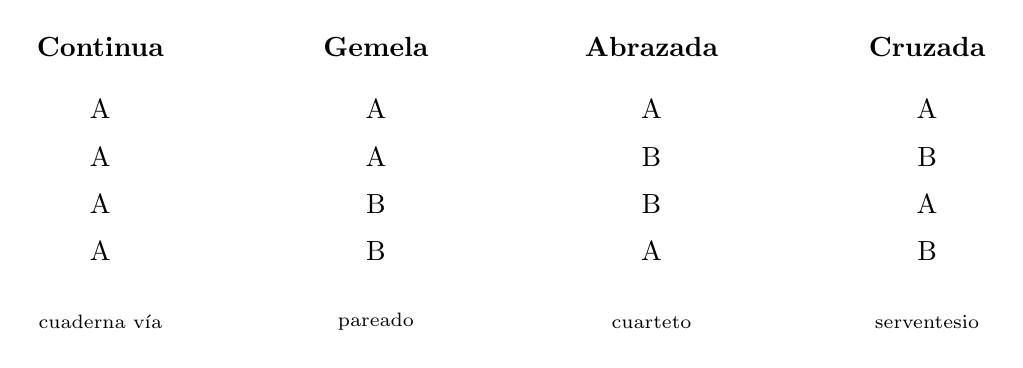
\begin{tikzpicture}

\node[font=\bfseries] at (1.5,3) {Continua};
\node at (1.5,2.2) {A};\node at (1.5,1.6) {A};\node at (1.5,1.0) {A};\node at (1.5,0.4) {A};
\node[font=\bfseries] at (5,3) {Gemela};
\node at (5,2.2) {A};\node at (5,1.6) {A};\node at (5,1.0) {B};\node at (5,0.4) {B};
\node[font=\bfseries] at (8.5,3) {Abrazada};
\node at (8.5,2.2) {A};\node at (8.5,1.6) {B};\node at (8.5,1.0) {B};\node at (8.5,0.4) {A};
\node[font=\bfseries] at (12,3) {Cruzada};
\node at (12,2.2) {A};\node at (12,1.6) {B};\node at (12,1.0) {A};\node at (12,0.4) {B};
\node[font=\scriptsize, align=center] at (1.5,-0.5) {cuaderna vía};
\node[font=\scriptsize, align=center] at (5,-0.5) {pareado};
\node[font=\scriptsize, align=center] at (8.5,-0.5) {cuarteto};
\node[font=\scriptsize, align=center] at (12,-0.5) {serventesio};

\end{tikzpicture}
\end{document}
